% Provenance (never printed): see sources/outline_sources.md (Year 1:
% observational astronomy, photometry). Telescopes, angular resolution,
% gratings, the Doppler effect and the black-body laws are owned by the
% physics series and recalled here. Curves computed in
% figdata/bachelor-1/{blackbody_bands, extinction_line}.py; numbers of the
% exercises and problem in the Book 3 scratch calculator ch02.py.
\chapter{Telescopen, detectoren en fotometrie}\label{ch:b1:observing-the-sky}

Alles wat de sterrenkunde over de sterren weet, afgezien van een paar meteorieten
en de monsters die van de maan en van planetoïden zijn teruggebracht, heeft zij
uit het licht geleerd dat die sterren uitzenden. Dat licht gaat door de
atmosfeer van de aarde, die hele golflengtegebieden absorbeert en de rest
vervaagt; het wordt opgevangen door een spiegel wiens grootte beperkt hoe zwak
en hoe fijn de details kunnen zijn; het wordt geteld door een detector die
fotonen in elektronen omzet, en elke telling draagt een statistische
onzekerheid. Voordat een helderheid een \omterm{def:b1:observing-the-sky:flux}{lichtkracht} of een afstand wordt, moet
elk van deze stappen begrepen en gecorrigeerd zijn. Dit hoofdstuk volgt het
licht van de ster tot het getal: de vensters van de atmosfeer en de
extinctiewet, de telescoop en de \omterm{def:b1:observing-the-sky:seeing}{seeing}, de detector en zijn ruis, en daarna de
magnitudes, parallaxen en kleuren die gemeten flux omzetten in eigenschappen
van sterren. Dezelfde atmosfeer, van onderaf gezien, is het onderwerp van de
klimaathoofdstukken (\cref{ch:b1:radiation-heat-transport}); dezelfde fotometrie,
toegepast op planeten, opent het volgende hoofdstuk
(\cref{ch:b1:comparative-planetology}).

\begin{recall}
Het objectief van een telescoop, lens of spiegel, vangt licht op over zijn opening
en vormt een beeld in zijn brandpunt; diffractie door een opening met diameter
$D$ beperkt de kleinste hoek die hij nog scheidt tot ongeveer $1.22\,\lambda/D$,
het criterium van Rayleigh (het eerste jaar van de natuurkundeboeken). Een
tralie spreidt licht naar golflengte (tweede jaar), en een bron die langs de
kijklijn beweegt verschuift haar spectraallijnen door het Doppler-effect (klas~12). Een lichaam in thermisch evenwicht zendt het zwarte-lichaamspectrum uit,
waarvan de piek de wet van Wien volgt (tweede jaar). In de scheikunde groeit de
absorbantie van een oplossing evenredig met de weglengte.
\end{recall}

\section{De vensters van de atmosfeer}

De atmosfeer is voor sommige golflengten doorzichtig en voor andere ondoorzichtig.
Straling wordt vooral geabsorbeerd door waterdamp, koolstofdioxide en ozon, en
bij de kortste golflengten door de atomen en moleculen van de hoge atmosfeer zelf.
% ledger: nasa:ems-absorbers

\begin{definition}[Atmosferisch venster]\label{def:b1:observing-the-sky:window}
Een \emph{atmosferisch venster}\index{atmosferisch venster} is een golflengtegebied
waarin de atmosfeer het meeste van de straling doorlaat die haar bovenkant bereikt
tot aan de grond. Het \emph{optische venster} loopt van het nabije ultraviolet
tot het nabije infrarood; het \emph{radiovenster} van golflengten van ongeveer
een centimeter tot ongeveer tien meter.
\end{definition}

De figuur hieronder schetst de ondoorzichtigheid van de atmosfeer van gammastraling
tot lange radiogolven. Gammastraling, röntgenstraling en ultraviolet beneden ongeveer
\qty{0.3}{\micro\metre} bereiken de grond nooit: men waarneemt ze vanuit de ruimte.
Zichtbaar licht gaat erdoor, met enige vervaging. Het meeste infrarood wordt
geabsorbeerd door waterdamp en koolstofdioxide, behalve in smalle vensters die
grondobservatoria op hoge, droge plaatsen benutten; de \omterm{def:b1:observing-the-sky:magnitude}{fotometrische banden} van
het nabije infrarood liggen erin, bij \qty{1.24}{\micro\metre},
\qty{1.65}{\micro\metre} en \qty{2.16}{\micro\metre}. Golflengten van ongeveer
\qty{30}{\micro\metre} tot een millimeter worden weer geblokkeerd; radiogolven van
enkele centimeters tot ongeveer tien meter gaan erdoor, zelfs door wolken; langere
worden door de ionosfeer teruggekaatst.
% ledger: nasa:opacity-windows, baldry:2mass-pivot

\begin{omfigure}
\begin{tikzpicture}[x=1.0cm, y=2.2cm, font=\scriptsize]
% x = log10(lambda / 1 m) + 10 ; opacity 0..1 (schematic, after the NASA figure)
\fill[omSea!20] (0,0) rectangle (13,1.05);
\fill[brown!50] (0,0) -- (0,1) -- (3.45,1) -- (3.52,0.05) -- (4.03,0.05)
  -- (4.06,0.6) -- (4.09,0.15) -- (4.15,0.6) -- (4.22,0.15) -- (4.28,0.6)
  -- (4.34,0.15) -- (4.42,0.7) -- (4.55,0.25) -- (4.65,0.8) -- (4.9,0.2)
  -- (5.12,0.2) -- (5.25,0.7) -- (5.4,1) -- (7.0,1) -- (7.3,0.6) -- (7.6,0.75)
  -- (8.0,0.5) -- (8.5,0.03) -- (11.0,0.03) -- (11.3,1) -- (13,1) -- (13,0)
  -- cycle;
\draw[black!70] (0,0) rectangle (13,1.05);
\foreach \x in {0,...,13} { \draw (\x,0) -- (\x,-0.05); }
\foreach \x/\l in {0/0.1 nm, 2/10 nm, 4/1 \unit{\micro m}, 6/100 \unit{\micro m}, 8/1 cm,
  10/1 m, 12/100 m}
  { \node[below] at (\x,-0.05) {\l}; }
\foreach \y/\l in {0/0, 0.5/50, 1/100}
  { \draw (0,\y) -- (-0.1,\y); \node[left] at (-0.1,\y) {\l}; }
\node[rotate=90] at (-0.75,0.5) {ondoorzichtigheid (\%)};
\node at (6.5,-0.42) {\small golflengte (logaritmische schaal)};
\node[align=center] at (1.7,0.75) {gammastraling, röntgenstraling,\\ ultraviolet};
\node[align=center] at (6.2,0.75) {ver\\ infrarood};
\node[align=center] at (9.75,0.5) {radiovenster};
\node[omThm] at (4.15,0.86) {J H K};
\draw[-{Stealth}] (2.6,1.25) node[above] {optisch venster} -- (3.75,1.07);
\draw[-{Stealth}] (5.9,1.25) node[above] {infraroodvensters} -- (4.6,1.07);
\end{tikzpicture}

{\small De ondoorzichtigheid van de atmosfeer voor straling die uit de ruimte komt,
van \qty{0.1}{nm} tot \qty{1}{km} (logaritmische schaal). Schematisch, naar een
NASA-figuur in het publieke domein: alleen de vensters doen ertoe, niet de precieze
vorm van elke absorptieband. J, H en K markeren de \omterm{def:b1:observing-the-sky:magnitude}{fotometrische banden} van het
nabije infrarood.}
% ledger: nasa:opacity-windows, nasa:ems-absorbers, baldry:2mass-pivot
\end{omfigure}

\subsection*{Extinctie}

Ook binnen het optische venster verwijdert de atmosfeer een deel van het licht,
door absorptie en door verstrooiing aan moleculen en aerosolen. Een dunne laag
met dikte $\mathrm ds$ langs de straal verwijdert een deel van de intensiteit dat
evenredig is met $\mathrm ds$: $\mathrm dI = -\kappa I\,\mathrm ds$, waarin de
\omterm{def:b1:observing-the-sky:extinction}{extinctiecoëfficiënt} $\kappa$ (per meter) afhangt van de golflengte en van de
samenstelling van de lucht op die hoogte. Dit is de wet van de absorbantie van een
oplossing, toegepast op een luchtkolom.

\begin{proposition}[De wet van Bouguer]\label{prop:b1:observing-the-sky:bouguer}
Langs een straal door een absorberend medium neemt de intensiteit af als
\[
  I = I_0\,e^{-\tau}, \qquad \tau = \int_0^s \kappa\,\mathrm ds' ,
\]
waarin $I_0$ de intensiteit is die het medium binnenkomt en $\tau$, de optische
diepte van het pad, een zuiver getal is.
Voor een vlakparallelle atmosfeer wordt een ster op zenithoek $z$ (de hoek tussen
haar richting en de verticaal) gezien door de optische diepte $\tau(z) = \tau_0\sec z$,
waarin $\tau_0$ de optische diepte in het \omterm{def:b1:spherical-astronomy:celestial-sphere}{zenit} is.
\end{proposition}

\begin{proof}
De vergelijking $\mathrm dI/I = -\kappa\,\mathrm ds$ splitst zich; integreren vanaf de
bovenkant van de atmosfeer ($I = I_0$, $s = 0$) tot de waarnemer geeft
$\ln(I/I_0) = -\int_0^s\kappa\,\mathrm ds'$. In een vlakparallelle atmosfeer hangt
$\kappa$ alleen van de hoogte $y$ af, en een straal die onder $z$ ten opzichte van de
verticaal loopt, legt $\mathrm ds = \mathrm dy/\cos z$ af om $\mathrm dy$ te stijgen.
Dus $\tau(z) = \int \kappa(y)\,\mathrm dy/\cos z = \tau_0\sec z$.
\end{proof}

\begin{definition}[Luchtmassa, extinctiecoëfficiënt]\label{def:b1:observing-the-sky:extinction}
De \emph{luchtmassa}\index{luchtmassa} $X$ van een waarneming is de optische diepte
van de kijklijn gedeeld door de optische diepte in het \omterm{def:b1:spherical-astronomy:celestial-sphere}{zenit}: $X = \tau(z)/\tau_0$.
Zij is 1 in het \omterm{def:b1:spherical-astronomy:celestial-sphere}{zenit} en, voor een vlakparallelle atmosfeer, $X = \sec z$. De
\emph{extinctiecoëfficiënt}\index{extinctiecoëfficiënt} $k$ in een gegeven band
is de verzwakking, in magnitudes, die door één luchtmassa wordt veroorzaakt; zo
wordt een ster met magnitude $m_0$ boven de atmosfeer waargenomen als
\[
  m = m_0 + kX .
\]
\end{definition}

De magnitudes worden gedefinieerd in \cref{sec:b1:observing-the-sky:magnitudes}; hier
volstaat dat een verzwakking met de factor $e^{-\tau}$ $2.5\log_{10}e\;\tau = 1.086\,\tau$
magnitudes toevoegt, zodat $k = 1.086\,\tau_0$. De vlakparallelle \omterm{def:b1:observing-the-sky:extinction}{luchtmassa} is
uitstekend tot een hoogte van ongeveer \ang{30} ($X = 2$) en faalt nabij de
horizon, waar $\sec z$ onbeperkt groeit terwijl het werkelijke pad door een
gekromde atmosfeer eindig blijft; waarnemers vermijden daarom lage hoogten, ook
vanwege de vervaging die met het pad toeneemt.

\begin{method}[De extinctielijn]\label{met:b1:observing-the-sky:extinction-line}
Om de magnitude $m_0$ te vinden die een ster boven de atmosfeer zou hebben:
\begin{enumerate}
  \item meet de magnitude $m$ van de ster, of van een standaardster, bij
        verschillende \omterm{def:b1:observing-the-sky:extinction}{luchtmassa}'s gedurende de nacht, terwijl zij opkomt of ondergaat;
  \item bereken elke \omterm{def:b1:observing-the-sky:extinction}{luchtmassa} uit de zenithoek, $X = \sec z$;
  \item zet $m$ uit tegen $X$ en pas met de kleinste kwadraten een rechte lijn door de punten;
  \item de helling is de \omterm{def:b1:observing-the-sky:extinction}{extinctiecoëfficiënt} $k$ van die nacht in die band; het snijpunt
        bij $X = 0$ is $m_0$.
\end{enumerate}
Dezelfde $k$ corrigeert daarna elke andere ster die die nacht in dezelfde band is
waargenomen: $m_0 = m - kX$.
\end{method}

\begin{example}
Op een nacht werd een ster zes keer gemeten in de V-band:
\begin{center}
\small
\begin{tabular}{lcccccc}
\hline
$X$ & 1.05 & 1.18 & 1.36 & 1.62 & 1.95 & 2.31 \\
$m$ & 8.024 & 8.031 & 8.072 & 8.104 & 8.171 & 8.216 \\
\hline
\end{tabular}
\end{center}
De kleinste-kwadratenlijn, in de figuur hieronder getekend, heeft helling
$k = \qty{0.160}{\mag}$ per \omterm{def:b1:observing-the-sky:extinction}{luchtmassa} en snijpunt $m_0 = 7.851$. De punten
verspreiden zich eromheen met \num{0.006} magnitudes, de precisie van een goede
nachtelijke fotometrie. In het \omterm{def:b1:spherical-astronomy:celestial-sphere}{zenit} wordt de ster met \num{0.16} magnitudes
verzwakt, een verlies van $1 - 10^{-0.4\times0.160} = \qty{14}{\percent}$ van haar licht.
\end{example}

\begin{omfigure}
\begin{tikzpicture}
\begin{axis}[omrecord, width=0.62\linewidth, height=5.4cm, xmin=0, xmax=2.5,
  ymin=7.80, ymax=8.28, y dir=reverse, xlabel={luchtmassa $X$},
  ylabel={magnitude $m$}, yticklabel style={/pgf/number format/fixed,
  /pgf/number format/precision=2}, tick label style={font=\scriptsize},
  label style={font=\small}]
\addplot[omThm, line width=0.9pt, dashed] table[x=X, y=m] {figdata/out/bachelor-1-extinction_line-fit.dat};
\addplot[only marks, mark=*, mark size=1.6pt, omDef] table[x=X, y=m] {figdata/out/bachelor-1-extinction_line-obs.dat};
\node[font=\scriptsize, right, fill=white, inner sep=1pt] at (axis cs:0.05,7.83) {$m_0 = 7.851$};
\node[font=\scriptsize, fill=white, inner sep=1pt, rotate=-10] at (axis cs:0.95,8.10) {helling $k = 0.160$};
\end{axis}
\end{tikzpicture}

{\small Een extinctielijn: de magnitude van één ster bij zes \omterm{def:b1:observing-the-sky:extinction}{luchtmassa}'s (puntjes)
en de kleinste-kwadratenlijn, geëxtrapoleerd tot $X = 0$, de magnitude boven de
atmosfeer. Magnitudes nemen naar beneden toe: een zwakkere ster ligt lager.}
\end{omfigure}

\subsection*{Turbulentie in de atmosfeer}

De lucht boven een telescoop is nooit stil. Cellen lucht met iets verschillende
temperaturen, en dus met iets verschillende brekingsindices, drijven over de
bundel en buigen die over kleine willekeurige hoeken, en dat verandert vele malen
per seconde. Het oog ziet een ster fonkelen; een lange belichting legt een vervaagde
vlek vast die veel groter is dan het diffractiepatroon van de telescoop.

\begin{definition}[Atmosferische turbulentie]\label{def:b1:observing-the-sky:seeing}
De \emph{seeing}\index{seeing} op een plaats is de hoekdiameter van het beeld van een
puntbron, vervaagd door atmosferische turbulentie bij een lange belichting, gemeten
als de volle breedte op halve hoogte van het beeld, in boogseconden.
\end{definition}

De \omterm{def:b1:observing-the-sky:seeing}{seeing} verandert van nacht tot nacht en van uur tot uur. Plaatsen worden erop
gekozen: op de top van Maunakea, op \qty{4204}{m}, is de mediane \omterm{def:b1:observing-the-sky:seeing}{seeing} van de vrije
atmosfeer ongeveer \ang{;;0.40}, van ongeveer \ang{;;0.45} in de winter tot \ang{;;0.35}
in de zomer, met de beste tien procent van de nachten beneden ongeveer \ang{;;0.25};
dezelfde plaats heeft een mediaan van slechts \qty{0.9}{mm} neerslagbaar waterdamp
erboven, wat haar infraroodvensters opent.
% ledger: cfht:site, cfht:seeing

\section{Telescopen en scheidend vermogen}

Een telescoop doet twee dingen: hij vangt licht op over het oppervlak van zijn
objectief, en hij vormt een beeld waarin details worden gescheiden. Het
opvangoppervlak groeit als $D^2$: een spiegel die twee keer zo breed is, vangt
in dezelfde tijd vier keer zoveel fotonen op en bereikt sterren die vier keer zo
zwak zijn. Het scheidend vermogen wordt door diffractie begrensd tot ongeveer
$1.22\,\lambda/D$, en door de \omterm{def:b1:observing-the-sky:seeing}{seeing}.

\begin{example}
De Canada--France--Hawaii-telescoop op Maunakea heeft een opening van
\qty{3.58}{m}. Bij \qty{550}{nm} is haar diffractiegrens
\[
  1.22\times\frac{\qty{550e-9}{m}}{\qty{3.58}{m}} = \qty{1.87e-7}{rad}
  = \ang{;;0.039},
\]
ongeveer tien keer fijner dan de mediane \omterm{def:b1:observing-the-sky:seeing}{seeing} van \ang{;;0.40} op dezelfde
plaats. De twee grenzen zijn gelijk voor een spiegel met diameter $D = 1.22\lambda/\theta =
1.22\times\qty{550e-9}{m}/(\num{0.40}/\num{206265}) = \qty{0.35}{m}$: elke
grondtelescoop die breder is dan ongeveer \qty{35}{cm} wordt bij zichtbaar licht
door de \omterm{def:b1:observing-the-sky:seeing}{seeing} begrensd, niet door haar eigen optica.
% ledger: cfht:aperture, cfht:seeing
\end{example}

Een grote grondtelescoop wint dus opvangoppervlak, niet scherpte, tenzij hij de
turbulentie corrigeert. \emph{Adaptieve optica} doet dat: een sensor meet vele malen
per seconde hoe het golffront van een heldere ster (of van een kunstmatige ster die
door een laser in de hoge atmosfeer wordt opgewekt) vervormd is, en een dunne
spiegel, door veel kleine stellers gebogen, heft de vervorming op. De correctie werkt
het best in het infrarood, waar de turbulentie trager en zwakker is, en over een klein
veld rond de geleidester. In de ruimte is er helemaal geen \omterm{def:b1:observing-the-sky:seeing}{seeing}.

\section{Detectoren}

Het oog integreert licht gedurende een fractie van een seconde en reageert op een
klein deel van de fotonen die erin vallen. Fotografische platen integreerden uren lang,
maar registreerden slechts een klein deel van het licht. De moderne sterrenkunde
gebruikt fotondetectoren van halfgeleiders, waarin elk geabsorbeerd foton met genoeg
energie een elektron vrijmaakt.

\begin{definition}[Kwantumrendement, signaal-ruisverhouding]\label{def:b1:observing-the-sky:detector}
Het \emph{kwantumrendement}\index{kwantumrendement} $\eta$ van een detector bij een
gegeven golflengte is de fractie van de inkomende fotonen die hij registreert, als
fotoelektronen: $\eta = N_\mathrm{e}/N_\gamma$. De
\emph{signaal-ruisverhouding}\index{signaal-ruisverhouding} van een meting is het
gemeten signaal gedeeld door zijn standaardafwijking, de typische grootte van zijn
toevallige fout.
\end{definition}

De \emph{ladingsgekoppelde inrichting} (CCD) is de standaarddetector van het optische
venster. Het is een dunne plak silicium, verdeeld in een raster van pixels, elk een
potentiaalput die de elektronen opslaat die tijdens de belichting door de daarin
geabsorbeerde fotonen zijn vrijgemaakt. Aan het eind van de belichting schuiven
spanningen die na elkaar op de elektroden worden gezet de ladingen van pixel tot pixel,
rij na rij, naar één versterker die ze één voor één meet; het beeld is de tabel van de
tellingen. Een CCD registreert een groot deel van de invallende fotonen over het
grootste deel van het zichtbare licht, zijn respons is evenredig met het ontvangen licht
tot een maximale lading per pixel (zijn \emph{volle put}), en hij kan uren integreren.
Infraroodmatrices werken volgens hetzelfde principe met andere halfgeleiders, pixel
voor pixel uitgelezen.

Fotonen komen willekeurig aan. Als een bron gemiddeld $N$ fotoelektronen tijdens een
belichting levert, fluctueert de werkelijk geregistreerde telling van de ene belichting
tot de volgende met de standaardafwijking $\sqrt N$ (Poisson-statistiek, die uit de
kansrekening wordt overgenomen: de tellingen van zeldzame onafhankelijke gebeurtenissen).

\begin{proposition}[Fotonruis]\label{prop:b1:observing-the-sky:snr}
Wanneer het fotonruis van de bron alleen overheerst, wordt een bron die $R$
fotoelektronen per seconde levert, in een tijd $t$ gemeten met de
\omterm{def:b1:observing-the-sky:detector}{signaal-ruisverhouding}
\[
  \mathrm{SNR} = \frac{Rt}{\sqrt{Rt}} = \sqrt{Rt} ;
\]
zij groeit met de wortel uit de belichtingstijd, en met de diameter van de telescoop
(omdat $R \propto D^2$). De fout op de magnitude is dan $\sigma_m \approx 1.086/\mathrm{SNR}$.
\end{proposition}

\begin{proof}
Het signaal is $N = Rt$ en de standaardafwijking $\sqrt N$. Voor de magnitude geldt
$m = -2.5\log_{10}N + \text{constante}$, dus een kleine fout $\sigma_N$ geeft
$\sigma_m = 2.5\log_{10}e\;\sigma_N/N = 1.086/\mathrm{SNR}$.
\end{proof}

Om een magnitude tot op \num{0.01} te meten, is een SNR van ongeveer 109 nodig, dat wil
zeggen ongeveer \num{12000} fotoelektronen. Bij zwakke bronnen spelen twee andere
termen mee. De hemel zelf gloeit, en elke pixel van het beeld van de ster verzamelt ook
hemelfotonen, met een snelheid $B$; en de versterker voegt aan elke uitgelezen pixel
een uitleesruis $\sigma_r$ toe. De volledige uitdrukking,
\[
  \mathrm{SNR} = \frac{Rt}{\sqrt{Rt + Bt + n\sigma_r^2}}
\]
over de $n$ pixels van het beeld, wordt $\sqrt{Rt}$ voor een heldere ster en
$R\sqrt t/\sqrt B$ voor een bron die zwakker is dan de hemel. Omdat $B$ groeit met de
oppervlakte van de seeingschijf, loont goede \omterm{def:b1:observing-the-sky:seeing}{seeing} dubbel: een scherper beeld scheidt
meer en verzamelt minder hemellicht (\cref{exo:b1:observing-the-sky:11}).

\begin{inthefield}[Een nacht bij de telescoop]
Fotometrie gebeurt met kalibraties evenzeer als met sterren. Voor de nacht neemt een
waarnemer op een professioneel observatorium \emph{bias}-opnamen (opnamen van nul
seconden, die de elektronische offset van elke pixel vastleggen) en \emph{flatfields}
(beelden van het gelijkmatig verlichte binnenste van de koepel of van de schemering,
die in kaart brengen hoe de gevoeligheid van pixel tot pixel en over het veld varieert);
de wetenschappelijke beelden worden gecorrigeerd door de bias af te trekken en door de
flat te delen. Gedurende de nacht worden standaardsterren met bekende magnitudes bij
verschillende \omterm{def:b1:observing-the-sky:extinction}{luchtmassa}'s waargenomen, om de extinctielijn en het nulpunt vast te
leggen dat tellingen in magnitudes omzet. Een nacht heet \emph{fotometrisch} wanneer de
extinctie stabiel genoeg blijft om deze correctie te laten gelden; op de top van
Maunakea zijn \qty{55}{\percent} van de nachten fotometrisch.
% ledger: cfht:nights
\begin{center}
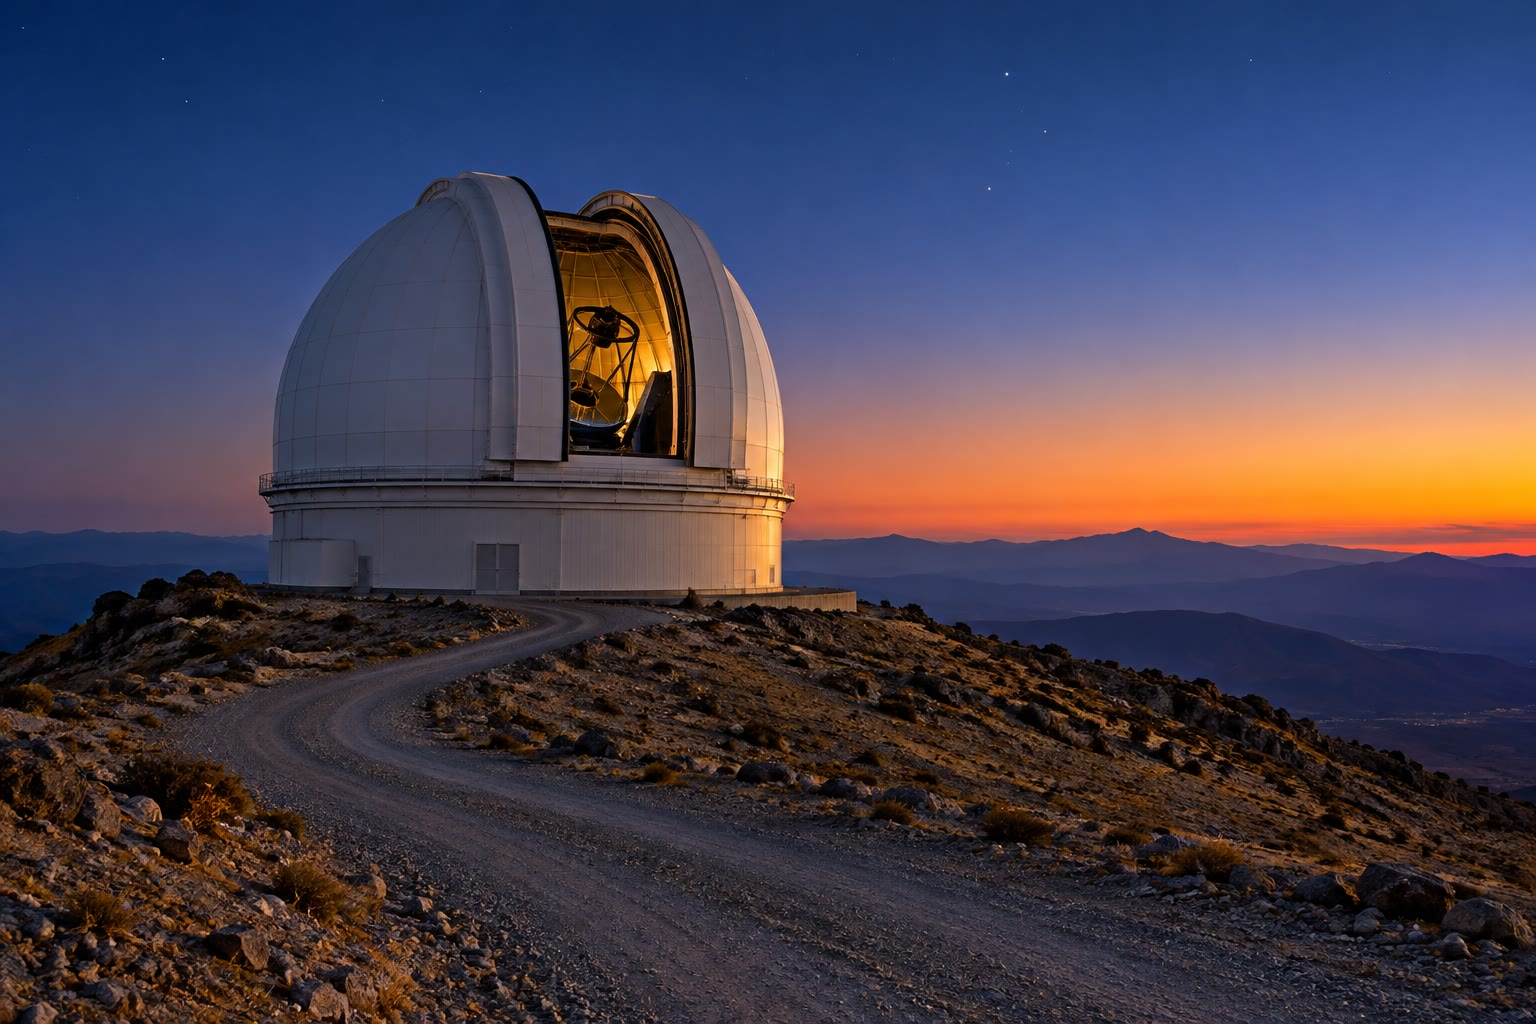
\includegraphics[width=0.55\linewidth]{images/book3/ai/b1-observatory-dusk.jpg}
\end{center}
\end{inthefield}

\section{Flux en magnitudes}\label{sec:b1:observing-the-sky:magnitudes}

\begin{definition}[Flux, lichtkracht]\label{def:b1:observing-the-sky:flux}
De \emph{flux}\index{flux (van een bron)} $F$ die van een bron wordt ontvangen, is het
vermogen van haar straling dat een eenheidsoppervlak loodrecht op haar richting
doorkruist, in watt per vierkante meter; beperkt tot een golflengteband is het de flux
in die band. De \emph{lichtkracht}\index{lichtkracht} $L$ van de bron is het totale
vermogen dat zij uitstraalt, in watt.
\end{definition}

\begin{proposition}[Kwadratenwet van de afstand]\label{prop:b1:observing-the-sky:inverse-square}
Een bron met \omterm{def:b1:observing-the-sky:flux}{lichtkracht} $L$ die in alle richtingen gelijk straalt, geeft, gezien op
afstand $d$ door de lege ruimte, de flux
\[
  F = \frac{L}{4\pi d^2} .
\]
\end{proposition}

\begin{proof}
In een stationaire toestand zonder absorptie is het vermogen dat elke bol rond de bron
doorkruist hetzelfde, $L$, door behoud van energie. Uit symmetrie is het gelijkmatig
verspreid over het oppervlak $4\pi d^2$ van de bol.
\end{proof}

\begin{example}
De \omterm{def:b1:observing-the-sky:flux}{lichtkracht} van de zon is \qty{3.828e26}{W}. Op één astronomische eenheid,
\qty{1.496e11}{m}, is haar flux $\num{3.828e26}/(4\pi\times
(\num{1.496e11})^2) = \qty{1361}{W.m^{-2}}$: de zonnestraling die de aarde aan de
bovenkant van haar atmosfeer ontvangt.
% ledger: sun:L, const:au, earth:TSI
\end{example}

Fluxen beslaan een enorm bereik, en sterrenkundigen vergelijken ze op een logaritmische
schaal die is overgeërfd van de klassen waarin de met het blote oog zichtbare sterren
ooit werden ingedeeld: de helderste van de eerste magnitude, de zwakste van de zesde.

\begin{definition}[Schijnbare magnitude, fotometrische band]\label{def:b1:observing-the-sky:magnitude}
Een \emph{fotometrische band}\index{fotometrische band} is een golflengtegebied dat door
een standaardfilter wordt geselecteerd en met een letter wordt aangeduid: U (ultraviolet),
B (blauw), V (visueel), R (rood), I (nabij infrarood), en J, H, K in de infraroodvensters.
De \emph{schijnbare magnitude}\index{schijnbare magnitude} $m$ van een bron in een band
wordt uit haar flux $F$ in die band gedefinieerd door
\[
  m_1 - m_2 = -2.5\log_{10}\frac{F_1}{F_2} ,
\]
waarbij het nulpunt door standaardsterren wordt vastgelegd, dicht bij de magnitude van
de ster Vega in elke band. Een verschil van 5 magnitudes is precies een factor 100 in
flux; één magnitude is een factor $100^{1/5} = 2.512$. Helderdere bronnen hebben kleinere,
en soms negatieve, magnitudes.
\end{definition}

De pivotgolflengten van de standaardfilters U, B, V, R en I zijn
\qty{358.5}{nm}, \qty{437.1}{nm}, \qty{547.8}{nm}, \qty{650.4}{nm} en
\qty{802.0}{nm}.
% ledger: baldry:bessell-pivot
In de V-band heeft de zon de \omterm{def:b1:observing-the-sky:magnitude}{schijnbare magnitude} $-26.74$, Sirius, de helderste ster van
de nachtelijke hemel, $-1.46$, en Vega $0.03$. De zon is dus
$10^{0.4\times(26.74 - 1.46)} = \num{1.29e10}$ keer helderder dan Sirius aan onze hemel;
dat zegt nog niets over welke van de twee het meest straalt, waarvoor de afstanden nodig zijn.
% ledger: nasa:sun-V, simbad:sirius, simbad:vega

\subsection*{Parallax en de parsec}

Terwijl de aarde om de zon draait, lijkt een nabije ster te bewegen tegen de veel
verder weg staande achtergrondsterren, en in een jaar beschrijft zij een kleine ellips.
Die schijnbare beweging is de rechtstreekste meting van afstanden tussen sterren: zij
gebruikt de baan van de aarde als meetbasis.

\begin{definition}[Jaarlijkse parallax, parsec]\label{def:b1:observing-the-sky:parallax}
De \emph{jaarlijkse parallax}\index{jaarlijkse parallax} $p$ van een ster is de hoek die
door de straal van de baan van de aarde, één astronomische eenheid, bij de ster wordt
ingesloten, gezien loodrecht op de kijklijn; zij is de halve lange as van de jaarlijkse
ellips die de ster lijkt te beschrijven. De \emph{parsec}\index{parsec} (\unit{\parsec})
is de afstand waarop één astronomische eenheid één boogseconde onder een hoek ziet:
\[
  \qty{1}{\parsec} = \frac{\qty{1}{\au}}{\tan\ang{;;1}} = \qty{206265}{\au}
  = \qty{3.0857e16}{m} = \qty{3.2616}{\lightyear} .
\]
\end{definition}

Omdat $p$ klein is, geldt $\tan p \approx p$ in radialen, en volgt de afstand meteen:
\[
  d = \frac{\qty{1}{\au}}{\tan p} \quad\Longrightarrow\quad
  \frac{d}{\unit{\parsec}} = \frac{1}{p/\text{boogseconde}} .
\]
Sirius heeft een parallax van \ang{;;0.37921}, dus ligt zij op $1/0.37921 =
\qty{2.637}{\parsec}$, \qty{8.60}{\lightyear}. Zelfs de dichtstbijzijnde sterren hebben
parallaxen kleiner dan één boogseconde, kleiner dan de \omterm{def:b1:observing-the-sky:seeing}{seeing}: de parallax wordt gevonden
uit de verschuiving van het middelpunt van het beeld van de ster, dat veel fotonen veel
nauwkeuriger lokaliseren dan de breedte van het beeld. Een ruimtemissie die aan het eind
van dit hoofdstuk wordt beschreven, heeft op deze manier de posities van bijna twee
miljard objecten gemeten.
% ledger: simbad:sirius, const:au, esa:gaia

\begin{omfigure}
\begin{tikzpicture}[font=\small]
\draw[black!50] (0,0) ellipse (2.0cm and 0.55cm);
\fill[orange!80!black] (0,0) circle (3pt) node[below=3pt] {zon};
\fill[blue!70!black] (-2.0,0) circle (2pt) node[left, align=right] {aarde, zes\\ maanden later};
\fill[blue!70!black] (2.0,0) circle (2pt) node[right] {aarde};
\fill (0,4.4) circle (1.6pt) node[above] {ster};
\draw[omDef, thick] (0,0) -- node[right, pos=0.55] {$d$} (0,4.4);
\draw[omThm] (2.0,0) -- (0,4.4);
\draw[omThm, dashed] (-2.0,0) -- (0,4.4);
\draw[thick] (0,0) -- node[above] {\qty{1}{\au}} (2.0,0);
\draw[omThm] (0,3.75) arc[start angle=-90, end angle=-65.6, radius=0.65cm];
\node[omThm] at (0.17,3.38) {$p$};
\end{tikzpicture}

{\small \omterm{def:b1:observing-the-sky:parallax}{Jaarlijkse parallax} (niet op schaal): vanaf de ster gezien sluit de
straal van de baan van de aarde de hoek $p$ in. Zes maanden later verschilt de richting van
de ster met $2p$. De echte hoek voor de dichtstbijzijnde ster is kleiner dan één boogseconde.}
\end{omfigure}

\begin{definition}[Absolute magnitude, afstandsmodulus]\label{def:b1:observing-the-sky:absolute}
De \emph{absolute magnitude}\index{absolute magnitude} $M$ van een ster in een band is de
\omterm{def:b1:observing-the-sky:magnitude}{schijnbare magnitude} die zij zou hebben op de afstand van \qty{10}{\parsec}, gezien door de
lege ruimte. Het verschil $m - M$ is haar \emph{afstandsmodulus}\index{afstandsmodulus}.
\end{definition}

\begin{proposition}[De afstandsmodulus]\label{prop:b1:observing-the-sky:modulus}
Voor een ster op afstand $d$, gezien door de lege ruimte,
\[
  m - M = 5\log_{10}\frac{d}{\qty{10}{\parsec}} .
\]
Als het licht onderweg door $A$ magnitudes extinctie wordt verzwakt, geldt
$m - M = 5\log_{10}(d/\qty{10}{\parsec}) + A$. In een band is de verhouding van de
\omterm{def:b1:observing-the-sky:flux}{lichtkrachten} van twee sterren $L_1/L_2 = 10^{0.4(M_2 - M_1)}$.
\end{proposition}

\begin{proof}
Volgens de kwadratenwet van de afstand verhouden de flux op $d$ en de flux op
\qty{10}{\parsec} zich als $F(d)/F(\qty{10}{\parsec}) = (\qty{10}{\parsec}/d)^2$. De
definitie van magnitudes geeft $m - M = -2.5\log_{10}(\qty{10}{\parsec}/d)^2
= 5\log_{10}(d/\qty{10}{\parsec})$. Extinctie vermenigvuldigt de flux met
$10^{-0.4A}$, wat $A$ aan $m$ toevoegt. Op de gemeenschappelijke afstand van
\qty{10}{\parsec} zijn de fluxen in de verhouding van de \omterm{def:b1:observing-the-sky:flux}{lichtkrachten}, en
$M_1 - M_2 = -2.5\log_{10}(L_1/L_2)$.
\end{proof}

De zon heeft de \omterm{def:b1:observing-the-sky:absolute}{absolute magnitude} $M_\odot = 4.83$ en de \omterm{def:b1:observing-the-sky:flux}{lichtkracht}
\qty{3.828e26}{W}. Door de \omterm{def:b1:observing-the-sky:absolute}{absolute magnitude} van een ster in V met die van de zon te
vergelijken, krijgt men haar \omterm{def:b1:observing-the-sky:flux}{lichtkracht} in V in zonne-eenheden,
$L/L_\odot = 10^{0.4(4.83 - M)}$ --- een \emph{V-band}-lichtkracht, want een ster die veel
heter of kouder is dan de zon, zendt een ander deel van haar vermogen buiten de V-band uit.
% ledger: sun:Mabs, sun:L

\subsection*{Kleur}

\begin{definition}[Kleurindex]\label{def:b1:observing-the-sky:colour-index}
De \emph{kleurindex}\index{kleurindex} van een ster is het verschil van haar magnitudes in
twee banden, de blauwste eerst; de meest gebruikte is $B - V$. Een kleine of negatieve
$B - V$ duidt op een blauwe ster, een grote op een rode ster.
\end{definition}

De \omterm{def:b1:observing-the-sky:colour-index}{kleurindex} hangt niet af van de afstand, omdat de kwadratenwet beide banden even sterk
verzwakt; zij meet de vorm van het spectrum, en dus de temperatuur van het oppervlak van de
ster. Een ster straalt ruwweg als een zwart lichaam waarvan het spectrum zijn piek heeft bij
$\lambda_\mathrm{max} = b/T$ (de wet van Wien, met $b = \qty{2.898e-3}{m.K}$, die uit het
tweede jaar van de natuurkundeboeken wordt overgenomen). De figuur hieronder tekent drie
zwartelichaamspectra: een koud lichaam van \qty{3500}{K} heeft zijn piek in het nabije
infrarood en geeft meer flux in V dan in B; de effectieve temperatuur van de zon,
\qty{5772}{K}, legt haar piek op \qty{502}{nm}, tussen B en V; een lichaam van
\qty{10000}{K} heeft zijn piek in het ultraviolet en is in B helderder dan in V. De verhouding
van de B- en V-stralingsintensiteiten stijgt gestaag met de temperatuur, van \num{0.46} tot
\num{0.97} en \num{1.53} voor de drie krommen, en dat is waarom $B - V$ daalt wanneer $T$
stijgt.
% ledger: const:b, nasa:sun-Teff, baldry:bessell-pivot

\begin{omfigure}
\begin{tikzpicture}
\begin{axis}[omrecord, width=0.9\linewidth, height=5.8cm, xmin=200, xmax=1500,
  ymin=0, ymax=1.17, xtick={200,400,...,1400}, ytick={0,0.5,1},
  xlabel={golflengte (nm)},
  ylabel={$B_\lambda$ / maximumwaarde}, tick label style={font=\scriptsize},
  label style={font=\small}, legend style={font=\scriptsize, at={(0.5,1.03)},
  anchor=south, draw=none, fill=none}, legend columns=3]
\addplot[red!75!black, line width=1.1pt] table[x=lam_nm, y=t3500] {figdata/out/bachelor-1-blackbody_bands-curves.dat};
\addplot[orange!90!black, line width=1.1pt] table[x=lam_nm, y=t5772] {figdata/out/bachelor-1-blackbody_bands-curves.dat};
\addplot[omDef, line width=1.1pt] table[x=lam_nm, y=t10000] {figdata/out/bachelor-1-blackbody_bands-curves.dat};
\legend{\qty{3500}{K}, \qty{5772}{K} (de zon), \qty{10000}{K}}
\draw[black!45, densely dashed] (axis cs:358.5,0) -- (axis cs:358.5,1.06);
\node[font=\scriptsize, above, inner sep=1pt] at (axis cs:358.5,1.06) {U};
\draw[black!45, densely dashed] (axis cs:437.1,0) -- (axis cs:437.1,1.06);
\node[font=\scriptsize, above, inner sep=1pt] at (axis cs:437.1,1.06) {B};
\draw[black!45, densely dashed] (axis cs:547.8,0) -- (axis cs:547.8,1.06);
\node[font=\scriptsize, above, inner sep=1pt] at (axis cs:547.8,1.06) {V};
\draw[black!45, densely dashed] (axis cs:650.4,0) -- (axis cs:650.4,1.06);
\node[font=\scriptsize, above, inner sep=1pt] at (axis cs:650.4,1.06) {R};
\draw[black!45, densely dashed] (axis cs:802.0,0) -- (axis cs:802.0,1.06);
\node[font=\scriptsize, above, inner sep=1pt] at (axis cs:802.0,1.06) {I};
\end{axis}
\end{tikzpicture}

{\small Zwartelichaamspectra bij drie temperaturen, elk gedeeld door het eigen maximum, met
de pivotgolflengten van de U-, B-, V-, R- en I-filters (gestreept). De piek verschuift naar
kortere golflengten naarmate de temperatuur stijgt (de wet van Wien): \qty{828}{nm},
\qty{502}{nm} en \qty{290}{nm}.}
% ledger: const:h, const:c, const:kB, const:b, nasa:sun-Teff, baldry:bessell-pivot
\end{omfigure}

Vier heldere sterren laten het bereik van kleuren zien:
\begin{center}
\small
\begin{tabular}{lcccc}
\hline
ster & $V$ & $B$ & $B - V$ & parallax (\unit{mas}) \\
\hline
Rigel & 0.13 & 0.10 & $-0.03$ & 3.78 \\
Altair & 0.76 & 0.98 & 0.22 & 194.95 \\
Polaris & 2.02 & 2.62 & 0.60 & 7.54 \\
Betelgeuse & 0.42 & 2.27 & 1.85 & 6.55 \\
\hline
\end{tabular}
\end{center}
% ledger: simbad:rigel, simbad:altair, simbad:polaris, simbad:betelgeuse
Rigel is blauwwit en Betelgeuse, in hetzelfde sterrenbeeld, oranjerood: een kleurverschil dat
met het blote oog zichtbaar is. Hun spectraaltypen, B8 en M1--M2, zeggen hetzelfde in de taal
van de spectra, het onderwerp van Boek 5.

\section{Spectrografen}

Fotometrie meet het licht in enkele brede banden; een spectrograaf spreidt het uit tot een
spectrum. Licht uit het brandpunt van de telescoop gaat door een smalle spleet, wordt
evenwijdig gemaakt door een collimator, wordt door een tralie (of een prisma) gespreid en
door een camera op de detector gefocusseerd, waar elke golflengte op een andere kolom van
pixels valt (zie de figuur hieronder). Een tralie met $N$ verlichte lijnen, in de orde $k$
gebruikt, scheidt twee golflengten die $\Delta\lambda$ uit elkaar liggen wanneer
$\lambda/\Delta\lambda \le kN$, zijn scheidend vermogen (dat uit het tweede jaar van de
natuurkundeboeken wordt herhaald).

\begin{omfigure}
\begin{tikzpicture}[font=\scriptsize, >=Stealth]
\draw[thick, fill=omSea!25] (0.15,0) ellipse (0.13 and 0.9);
\node[below] at (0.15,-0.95) {objectief};
\draw[omDef] (-1.3,0.75) -- (0.15,0.75) -- (2.4,0);
\draw[omDef] (-1.3,-0.75) -- (0.15,-0.75) -- (2.4,0);
\draw[omDef, ->] (-1.3,0) -- (-0.2,0);
\node[above] at (-0.8,0.75) {sterrenlicht};
\draw[very thick] (2.4,-0.35) -- (2.4,-0.06); \draw[very thick] (2.4,0.06) -- (2.4,0.35);
\node[above] at (2.4,0.38) {spleet};
\draw[omDef] (2.4,0) -- (3.6,0.55); \draw[omDef] (2.4,0) -- (3.6,-0.55);
\draw[thick, fill=omSea!25] (3.6,0) ellipse (0.1 and 0.72); \node[below] at (3.6,-0.74) {collimator};
\draw[omDef] (3.6,0.55) -- (4.9,0.55); \draw[omDef] (3.6,-0.55) -- (4.9,-0.55);
\draw[thick, pattern=north east lines] (4.85,-0.8) rectangle (5.0,0.8);
\node[below] at (4.92,-0.82) {tralie};
\draw[blue!70!black] (5.0,0.3) -- (6.4,0.95); \draw[red!70!black] (5.0,0.3) -- (6.4,-0.15);
\draw[blue!70!black] (5.0,-0.3) -- (6.4,0.35); \draw[red!70!black] (5.0,-0.3) -- (6.4,-0.75);
\draw[thick, fill=omSea!25] (6.4,0.1) ellipse (0.1 and 1.08); \node[below] at (6.4,-1.0) {camera};
\draw[blue!70!black] (6.4,0.95) -- (7.6,0.55); \draw[blue!70!black] (6.4,0.35) -- (7.6,0.55);
\draw[red!70!black] (6.4,-0.15) -- (7.6,-0.45); \draw[red!70!black] (6.4,-0.75) -- (7.6,-0.45);
\fill[black!70] (7.6,-0.8) rectangle (7.75,0.9);
\node[right, align=left] at (7.8,0.05) {detector:\\ één golflengte\\ per kolom};
\end{tikzpicture}

{\small Het pad van het licht door een telescoop en een tralie-spectrograaf (schematisch,
met het objectief van de telescoop en de optiek als lenzen getekend, en twee golflengten):
de spleet isoleert het beeld van de ster, de collimator maakt de bundel evenwijdig, het tralie
spreidt haar, en de camera focusseert elke golflengte op een eigen plaats op de detector.}
\end{omfigure}

Een spectrum draagt drie soorten informatie. Zijn \emph{lijnen}, donker waar atomen en ionen
van de atmosfeer van de ster absorberen, helder waar een heet dun gas uitstraalt, bepalen
welke scheikundige elementen aanwezig zijn. De vorm van zijn continuüm en de relatieve sterkte
van lijnen die bij verschillende temperaturen ontstaan, geven de temperatuur van het gas. En de
Doppler-verschuiving van de lijnen geeft de snelheid langs de kijklijn: een lijn met
rustgolflengte $\lambda$ verschuift met $\Delta\lambda = \lambda v_r/c$ voor een radiale
snelheid $v_r$ die veel kleiner is dan $c$. Om $v_r$ tot op \qty{1}{km.s^{-1}} te meten, is een
scheidend vermogen nodig van de orde van $c/v_r = \num{300000}$, of een matig scheidend vermogen
en veel lijnen samen gemeten. Hoe spectra de structuur, samenstelling en bewegingen van sterren
en sterrenstelsels onthullen, is het onderwerp van Boek 5.

\section{Waarnemen vanuit de ruimte}

Boven de atmosfeer zijn er geen gesloten vensters, geen extinctie, geen \omterm{def:b1:observing-the-sky:seeing}{seeing}, en in het
infrarood geen gloed van warme lucht. Ruimtetelescopen betalen daarvoor een prijs: de
beperkte massa en grootte die een raket kan lanceren, en, voor de meeste, de onmogelijkheid
van reparatie. Zij worden gebruikt waar de grond niet kan wedijveren: voor gammastraling,
röntgenstraling en ultraviolet licht, dat de grond nooit bereikt; voor het infrarood voorbij de
smalle vensters; voor beelden op de diffractiegrens over een groot veld; en voor metingen, zoals
de parallaxen van zeer veel sterren, die een stabiel instrument buiten de turbulente lucht vereisen.

\begin{dated}{2026}
% ledger: nasa:hubble-mirror, nasa:jwst-mirror, nasa:jwst-orbit, nasa:jwst-launch, nasa:jwst-range, esa:gaia
Drie ruimteobservatoria laten het bereik zien. De Hubble-ruimtetelescoop, in 1990 gelanceerd,
heeft een primaire spiegel van \qty{2.4}{m} doorsnede. De James Webb-ruimtetelescoop, op
25 december 2021 gelanceerd, heeft een primaire spiegel van \qty{6.5}{m} doorsnede, samengesteld
uit 18 zeshoekige segmenten, met een opvangoppervlak van \qty{25}{m^2}; hij werkt van
\qty{0.6}{\micro\metre} tot \qty{28.5}{\micro\metre} en draait om de zon nabij het tweede
Lagrangepunt, L2, \num{1.5} miljoen kilometer van de aarde, aan de kant die van de zon af ligt.
Gaia, op 19 december 2013 gelanceerd naar hetzelfde Lagrangepunt, L2, gebruikte twee telescopen op een
gemeenschappelijk brandvlak van CCD's om de posities en bewegingen van bijna twee miljard
objecten in drie dimensies in kaart te brengen; haar waarnemingen zijn afgerond en haar catalogi
worden nu vrijgegeven.
\end{dated}

\begin{omfigure}
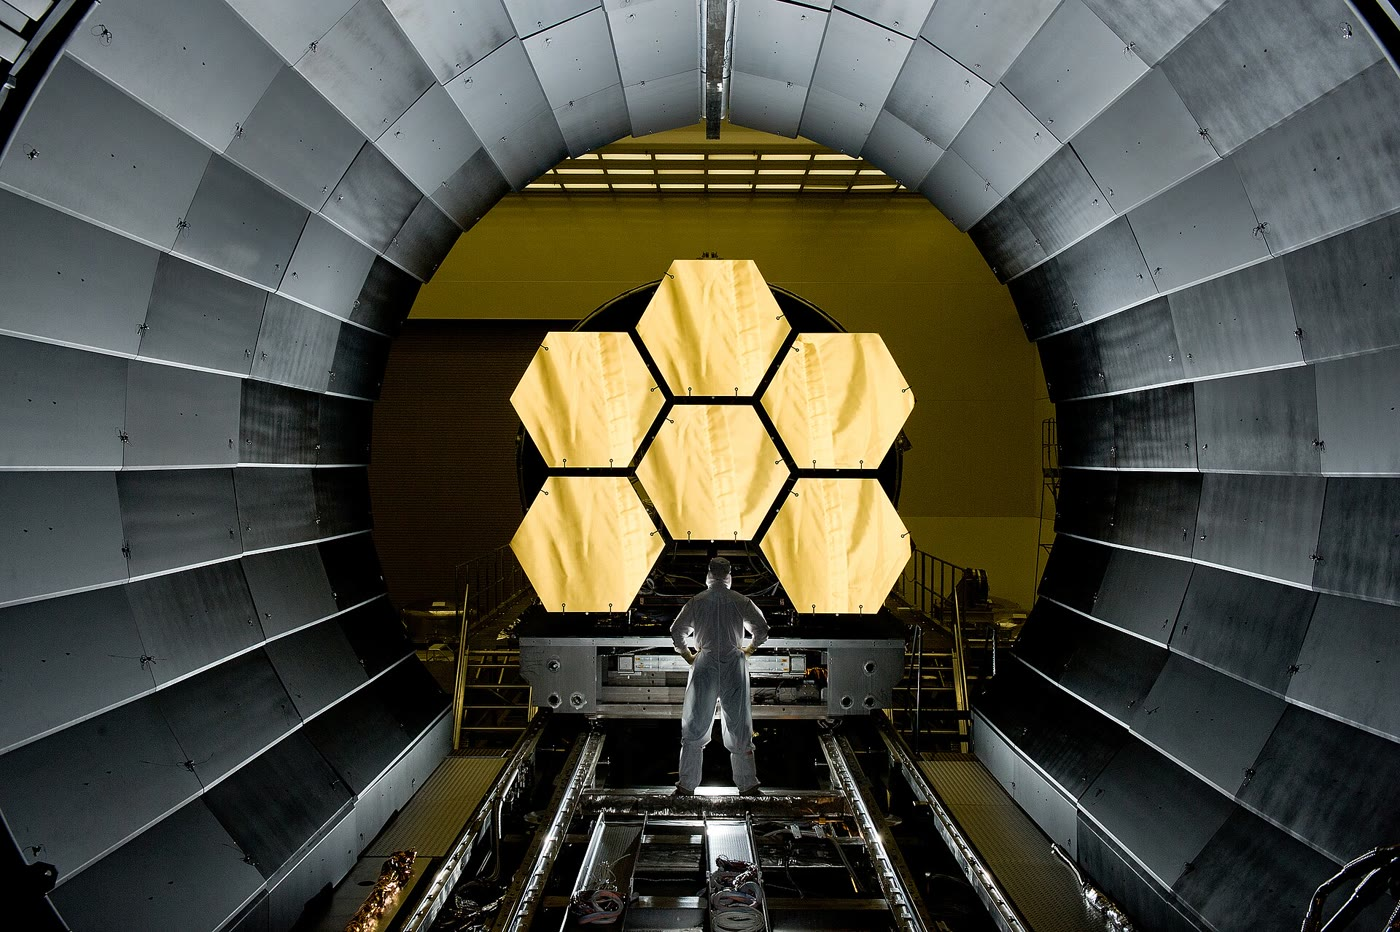
\includegraphics[width=0.78\linewidth]{images/book3/b1-jwst-mirror-segments.jpg}

{\small Zes van de 18 zeshoekige segmenten van de primaire spiegel van de James Webb-ruimtetelescoop,
voorbereid op koude tests in 2011; samen, uitgevouwen in de ruimte, vormen de 18 een spiegel van
\qty{6.5}{m} breed. Foto NASA/MSFC/David Higginbotham, publiek domein.}
% ledger: commons:jwst-mirror, nasa:jwst-mirror
\end{omfigure}

\section{Oefeningen}

\begin{exercise}[$\star$]\label{exo:b1:observing-the-sky:1}
Wat is de verhouding van de fluxen van twee sterren met magnitudes 1.0 en 6.0? Van
Rigel ($V = 0.13$) en Polaris ($V = 2.02$)? Welke is aan de hemel het helderst?
\end{exercise}

\begin{exercise}[$\star$]\label{exo:b1:observing-the-sky:2}
De parallax van Altair is \ang{;;0.19495}. Geef haar afstand in \omterm{def:b1:observing-the-sky:parallax}{parsecs}, in
astronomische eenheden en in lichtjaren.
\end{exercise}

\begin{exercise}[$\star$]\label{exo:b1:observing-the-sky:3}
Bereken de diffractiegrens van een ruimtetelescoop van \qty{2.4}{m} bij \qty{550}{nm}, in
boogseconden, en vergelijk die met een \omterm{def:b1:observing-the-sky:seeing}{seeing} van \ang{;;0.40}. Doe hetzelfde voor een telescoop
van \qty{6.5}{m} bij \qty{2.0}{\micro\metre}.
\end{exercise}

\begin{exercise}[$\star$]\label{exo:b1:observing-the-sky:4}
Rangschik uit de tabel van de vier heldere sterren Rigel, Altair, Polaris en Betelgeuse van het
heetste oppervlak naar het koelste. Waarom kan de \omterm{def:b1:observing-the-sky:colour-index}{kleurindex} tussen sterren op zeer
verschillende afstanden worden vergeleken?
\end{exercise}

\begin{exercise}[$\star\star$]\label{exo:b1:observing-the-sky:5}
Een ster wordt op dezelfde nacht gemeten met magnitude 6.412 bij een zenithoek van \ang{30} en
met 6.590 bij \ang{60}. Reken, uitgaande van een vlakparallelle atmosfeer, de twee \omterm{def:b1:observing-the-sky:extinction}{luchtmassa}'s,
de \omterm{def:b1:observing-the-sky:extinction}{extinctiecoëfficiënt} en de magnitude van de ster boven de atmosfeer uit.
\end{exercise}

\begin{exercise}[$\star\star$]\label{exo:b1:observing-the-sky:6}
Een ster levert 400 fotoelektronen in een belichting van \qty{10}{s}, en het fotonruis van de ster
alleen overheerst. Wat is de \omterm{def:b1:observing-the-sky:detector}{signaal-ruisverhouding}? Hoe lang moet men belichten om een SNR van 100
te bereiken? Om de magnitude tot op \num{0.01} te meten?
\end{exercise}

\begin{exercise}[$\star\star$]\label{exo:b1:observing-the-sky:7}
Rigel heeft $V = 0.13$ en een parallax van \ang{;;0.00378}. Verwaarloos de extinctie tussen haar en
ons, bereken haar afstand, haar \omterm{def:b1:observing-the-sky:absolute}{absolute magnitude} en haar \omterm{def:b1:observing-the-sky:flux}{lichtkracht} in V in
zonne-eenheden ($M_\odot = 4.83$).
\end{exercise}

\begin{exercise}[$\star\star$]\label{exo:b1:observing-the-sky:8}
Vergelijk het opvangoppervlak van een spiegel van \qty{2.4}{m} (negeer zijn centrale
verduistering) met dat van de Webb-telescoop (\qty{25}{m^2}). Hoeveel korter is de belichting
waarin de Webb-telescoop evenveel fotonen opvangt? Welk deel van een volledige schijf van
\qty{6.5}{m} doorsnede vertegenwoordigt zijn opvangoppervlak, en waarom is dat minder dan één?
\end{exercise}

\begin{exercise}[$\star\star$]\label{exo:b1:observing-the-sky:9}
(a) Bereken uit de \omterm{def:b1:observing-the-sky:flux}{lichtkracht} van de zon, \qty{3.828e26}{W}, haar flux op \qty{10}{\parsec}.
(b) De schijnbare en \omterm{def:b1:observing-the-sky:absolute}{absolute magnitudes} van de zon zijn $-26.74$ en $4.83$. Gebruik de
\omterm{def:b1:observing-the-sky:absolute}{afstandsmodulus} om de afstand tussen zon en aarde in astronomische eenheden terug te vinden.
\end{exercise}

\begin{exercise}[$\star\star\star$]\label{exo:b1:observing-the-sky:10}
Toon uit \cref{prop:b1:observing-the-sky:bouguer} aan dat $k =
2.5\log_{10}e\;\tau_0$. Bereken voor de nacht van de extinctielijn ($k =
\num{0.160}$) de optische diepte in het \omterm{def:b1:spherical-astronomy:celestial-sphere}{zenit} $\tau_0$ en de fractie van het licht dat
de telescoop in het \omterm{def:b1:spherical-astronomy:celestial-sphere}{zenit} en bij $X = 2.31$ bereikt. Wat voorspelt een vlakparallelle
atmosfeer voor de \omterm{def:b1:observing-the-sky:extinction}{luchtmassa} bij een zenithoek van \ang{85}, en waarom mag die waarde
niet worden vertrouwd?
\end{exercise}

\begin{exercise}[$\star\star\star$]\label{exo:b1:observing-the-sky:11}
Een zwak melkwegstelsel levert $R = 50$ fotoelektronen per seconde in een telescoop, en de
hemel in het oppervlak van zijn beeld levert $B = \num{2000}$ per seconde bij een \omterm{def:b1:observing-the-sky:seeing}{seeing} van
\ang{;;0.80}. De uitleesruis is verwaarloosbaar. (a) Hoe lang moet men belichten voor een SNR
van 10? (b) De hemel in het beeld groeit met het oppervlak van de seeingschijf. Herhaal voor een
\omterm{def:b1:observing-the-sky:seeing}{seeing} van \ang{;;0.40}. (c) Toon aan dat voor een bron die veel zwakker is dan de hemel, de
belichtingstijd die voor een gegeven SNR nodig is, varieert als $\theta^2/D^2$, waarin $\theta$ de
\omterm{def:b1:observing-the-sky:seeing}{seeing} is en $D$ de diameter van de telescoop.
\end{exercise}

\begin{exercise}[$\star\star\star$]\label{exo:b1:observing-the-sky:12}
Een tralie met 1200 lijnen per millimeter wordt over \qty{100}{mm} verlicht en in de eerste orde
gebruikt. (a) Wat is zijn scheidend vermogen, en het kleinste scheidbare golflengteverschil bij
\qty{550}{nm}? (b) Welke radiale snelheid komt overeen met dat verschil? (c) De aarde beweegt om
de zon met \qty{29.78}{km.s^{-1}}. Hoeveel kan die beweging een lijn bij \qty{550}{nm}
verschuiven, en hoeveel resolutie-elementen is dat? Wat moet een waarnemer die de snelheid van een
ster meet daarom doen?
% ledger: earth:vorb
\end{exercise}

\section{Probleem: Het licht van Sirius wegen}

\begin{problem}[{Weekendprobleem --- hoe ver Sirius staat, hoe helder zij lijkt en hoeveel fotonen zij uitzendt, en hoeveel zonnen zij overstraalt}]
\label{pb:b1:observing-the-sky:1}
% ledger: simbad:sirius, simbad:vega, simbad:sirius-b, nasa:sun-V, sun:Mabs, const:au
% numbers computed in the scratch calculator calc/ch02.py from the rounded data
Sirius, de helderste ster van de nachtelijke hemel, heeft een zwakke begeleider, de witte dwerg
Sirius~B. Gebruik de gegevens:
\begin{center}
\small
\begin{tabular}{lcc}
\hline
object & $V$ & parallax \\
\hline
Sirius & $-1.46$ & \ang{;;0.37921} \\
Sirius B & $8.44$ & --- \\
Vega & $0.03$ & \ang{;;0.13023} \\
de zon & $-26.74$ & --- \\
\hline
\end{tabular}
\end{center}
met $M_\odot = 4.83$ in V, $\qty{1}{\parsec} = \qty{206265}{\au} =
\qty{3.0857e16}{m} = \qty{3.2616}{\lightyear}$, en een \omterm{def:b1:observing-the-sky:extinction}{extinctiecoëfficiënt} $k = 0.15$ per
\omterm{def:b1:observing-the-sky:extinction}{luchtmassa} op het observatorium.

\medskip
\noindent\textbf{Deel I --- Hoe ver staat Sirius?}
\begin{enumerate}
  \item Bereken de afstand van Sirius in \omterm{def:b1:observing-the-sky:parallax}{parsecs}.
  \item Druk die uit in astronomische eenheden en in meters.
  \item Druk die uit in lichtjaren. Hoelang geleden verliet het licht dat wij vanavond zien Sirius?
  \item Welke totale hoek beschrijft de richting van Sirius in een jaar heen en weer? Vergelijk die
        met een \omterm{def:b1:observing-the-sky:seeing}{seeing} van \ang{;;0.40}. Waarom kan de uitslag toch tot een kleine fractie van de
        \omterm{def:b1:observing-the-sky:seeing}{seeing} worden gemeten?
  \item Als de parallax met \ang{;;0.001} verkeerd was, met welke fractie zou de afstand dan
        verkeerd zijn, en met hoeveel lichtjaren?
\end{enumerate}

\medskip
\noindent\textbf{Deel II --- Hoe helder lijkt zij?}
\begin{enumerate}[resume]
  \item Bereken de verhouding van de fluxen van Sirius en Vega in V.
  \item Bereken de verhouding van de fluxen van de zon en Sirius.
  \item Bereken de verhouding van de fluxen van Sirius en Sirius~B.
  \item Vanaf het Paranal-observatorium kruist Sirius de meridiaan op een hoogte van \ang{82.09}
        (\cref{ch:b1:spherical-astronomy}). Bereken de \omterm{def:b1:observing-the-sky:extinction}{luchtmassa}, de extinctie en de magnitude die
        op dat moment wordt gemeten.
  \item Herhaal bij een hoogte van \ang{30}. Welk deel van het licht gaat onderweg verloren?
  \item Waarom zou de formule $X = \sec z$ een waarnemer die Sirius meet kort nadat zij is opgekomen,
        op een dwaalspoor brengen?
\end{enumerate}

\medskip
\noindent\textbf{Deel III --- Fotonen tellen.}
Een camera op een telescoop van \qty{1}{m} registreert $\num{3.0e4}$ fotoelektronen per seconde van
een ster met magnitude $V = 10.0$, na correctie voor extinctie. Elke pixel houdt op zijn hoogst
$\num{1.0e5}$ elektronen vast (zijn volle put).
\begin{enumerate}[resume]
  \item Hoeveel fotoelektronen per seconde registreert de camera van Sirius~B?
  \item Hoe lange belichting geeft Sirius~B een SNR van 1000, met fotonruis van de ster alleen? Wat is
        dan de fout op haar magnitude?
  \item Hoeveel fotoelektronen per seconde registreert de camera van Sirius?
  \item Als \qty{20}{\percent} van het licht van Sirius in haar helderste pixel valt, hoe lang duurt het
        dan voordat die pixel vol is?
  \item Op het beeld leveren de zwakke vleugels van het beeld van Sirius bij de plaats van Sirius~B
        $10^{-4}$ van het licht van Sirius per pixel, en de helderste pixel van Sirius~B verzamelt
        \qty{20}{\percent} van haar eigen licht. Vergelijk de twee snelheden in die pixel.
  \item Wat is de langste belichting die die pixel niet verzadigt? Bereken de SNR van Sirius~B in die
        pixel bij een belichting van \qty{0.5}{s}, met het fotonruis van beide bronnen. Is Sirius~B
        detecteerbaar, en wat maakt haar moeilijk?
\end{enumerate}

\medskip
\noindent\textbf{Deel IV --- Hoeveel zonnen?}
\begin{enumerate}[resume]
  \item Bereken de \omterm{def:b1:observing-the-sky:absolute}{afstandsmodulus} van Sirius.
  \item Leid de \omterm{def:b1:observing-the-sky:absolute}{absolute magnitude} van Sirius in V af, op twee decimalen.
  \item Bereken de afstand en de \omterm{def:b1:observing-the-sky:absolute}{absolute magnitude} van Vega.
  \item Welke van Sirius en Vega is intrinsiek het helderst in V, en met welke factor?
  \item Welke \omterm{def:b1:observing-the-sky:magnitude}{schijnbare magnitude} zou de zon hebben gezien vanaf de afstand van Sirius? Als men 6.0
        neemt als de zwakste magnitude die op een donkere nacht met het blote oog zichtbaar is, zou
        zij dan zichtbaar zijn?
  \item Tot welke afstand zou Sirius met het blote oog zichtbaar blijven?
  \item Bereken de \omterm{def:b1:observing-the-sky:flux}{lichtkracht} van Sirius in V in zonne-eenheden: hoeveel zonnen overstraalt Sirius?
\end{enumerate}
\end{problem}
